\section{Guidance and Control}

\subsection{Long Range Controller}

% ----------------------------------------------------------------------

\begin{frame}{\thesection. \insertsection \ - \insertsubsection}
	The long range approach is regulated by
	\begin{enumerate}
		\item Proportional Navigation control to steer the MAV
		\item PD control for the approach velocity
	\end{enumerate}
\end{frame}

% ----------------------------------------------------------------------

\begin{frame}{\thesection. \insertsection \ - \insertsubsection}
	Proportional Navigation 
	\begin{align}
		a_{\perp} = - \lambda |\dot{u}| \frac{u}{|u|} \times \Omega,
\; \text{with } \Omega = \frac{u \times \dot{u}}{u \cdot u},
	\end{align}
	\begin{enumerate}
	\item[$a_{\perp}$] Commanded acceleration normal to the MAV's velocity
	\item[$\lambda$] Navigation gain
	\item[$u$] Relative position of the car w.r.t the MAV
	\item[$\dot{u}$] Relative velocity of the car w.r.t. the MAV
	\end{enumerate}
\end{frame}

% ----------------------------------------------------------------------

\begin{frame}{\thesection. \insertsection \ - \insertsubsection}
	Why True Proportional Navigation?
	\begin{enumerate}
		\item Simplest variant of Proportional Navigation that worked
		\item Car is assumed to move close to constant velocity
	\end{enumerate}
\end{frame}

% ----------------------------------------------------------------------

\begin{frame}{\thesection. \insertsection \ - \insertsubsection}
	Approach velocity PD control
	\begin{align}
		a_\parallel = K_{p\parallel} u + K_{d\parallel} \dot{u} 
	\end{align}
	\begin{enumerate}
		\item[$a_\parallel$] Acceleration parallel to the line of sight
		\item[$K_{p\parallel}$, $K_{d\parallel}$] Constant proportional and derivative gains
		\item[$u$] Relative position of the car w.r.t the MAV
		\item[$\dot{u}$] Relative velocity of the car w.r.t. the MAV \textit{projected on the line of sight vector}
	\end{enumerate}
\end{frame}

% ----------------------------------------------------------------------

\begin{frame}{\thesection. \insertsection \ - \insertsubsection}
	The complete controller is the combination of both acceleration components
	\begin{align}
		a = a_\perp + a_\parallel
	\end{align}
	We only navigate horizontally, thus the $z$-axis is disregarded.
\end{frame}

% ----------------------------------------------------------------------

\subsection{Close Range Controller}
\begin{frame}{\thesection. \insertsection \ - \insertsubsection}
	The close range approach is regulated by
	\begin{enumerate}
		\item Horizontal control : PD controller to match the velocity of the car
		\item Vertical Control : Constant descent velocity
	\end{enumerate}

	\begin{align}
		a = K_p u + K_d \dot{u}
	\end{align}
	\begin{enumerate}
		\item[$a$] MAV acceleration
		\item[$K_p$, $K_d$] Proportional and derivative gain
		\item[$u$] Relative position of the car w.r.t. the MAV 
	\end{enumerate}
\end{frame}

% ----------------------------------------------------------------------

\begin{frame}{\thesection. \insertsection \ - \insertsubsection}
	\begin{figure}
		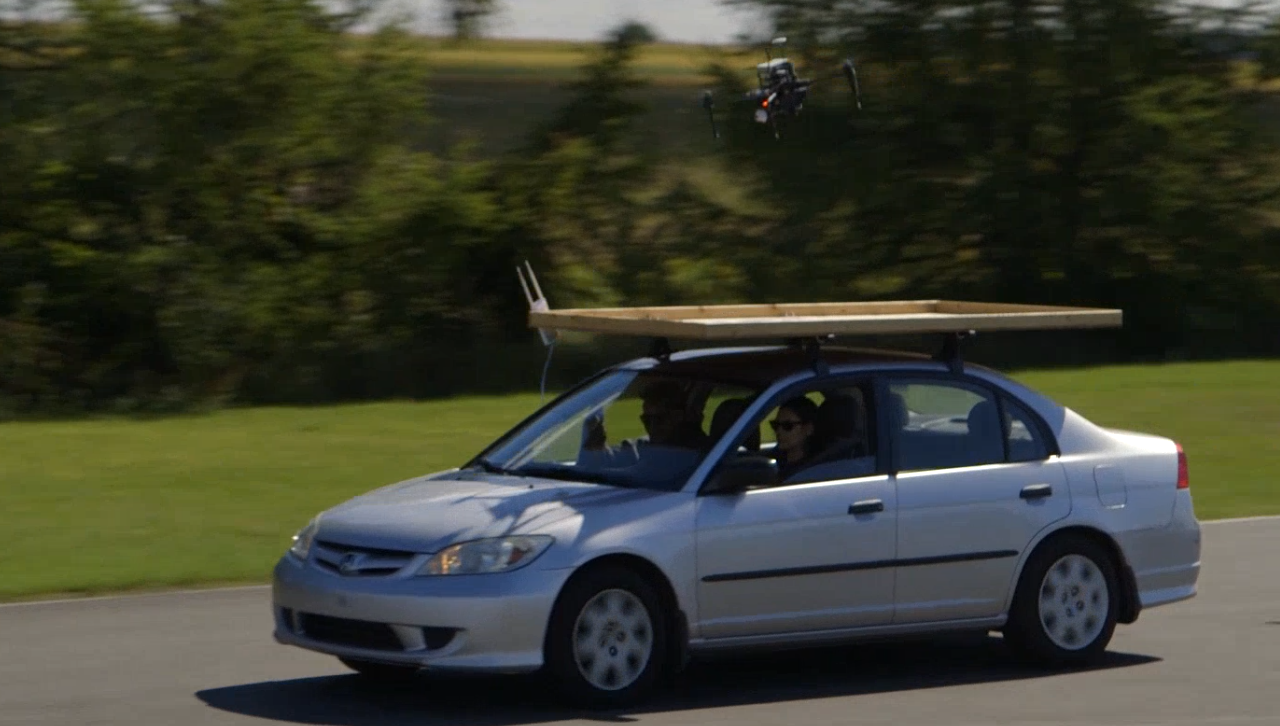
\includegraphics[width=0.7\paperwidth]{figures/landing.png}
		\caption{Descent begins when the MAV is stable over the landing platform. Constant vertical 
		velocity is applied. At $0.2$m the attitude is straighted out and the motors are cut off.}
	\end{figure}
\end{frame}


% ----------------------------------------------------------------------

\subsection{Controller Switching}
\begin{frame}{\thesection. \insertsection \ - \insertsubsection}
	We switch from long range PN to close range PID using a distance threshold. This distance
	is tuned such that
	\begin{enumerate}
		\item Visual detection of the AprilTag is acquired
		\item The outputs of both controllers are similar
	\end{enumerate}
	
\end{frame}

% ----------------------------------------------------------------------